\documentclass{article}
\usepackage{graphicx}
\usepackage{amssymb}
\usepackage{hyperref} 

\usepackage[capitalize]{cleveref}



\title{Deep Learning Final Project Report}
\author{Alon Malka \and Amit Arad }
\date{February 2026}

\begin{document}

\maketitle

\begin{abstract}
Music Source Separation (MSS) is the task of isolating an individual sound source from a mixed audio. This project implements and compares neural network architectures for spectrogram-based vocal separation: U-Net codecs and LSTM-based models. All operated on the log-magnitude spectrograms of the data and trained via curriculum learning ($2 \rightarrow 1$ into $4 \rightarrow 3$ source separation). Our results show that U-Net models outperform the LSTM baseline across all separation quality metrics (SDR, SIR, SAR). Additionally, we experimented with adding attention mechanisms to the Codec.
\end{abstract}


\section{Introduction}

Vocal separation is a sub-task of Music Source Separation (MSS), which means decomposing a mixed audio signal into its separate tracks (vocals, guitars, piano, etc.) It is still being researched and is our main objective in the final project.
Our preliminary work was to examine recent works and research in the field. We concluded that most approaches use U-Nets or LSTMs based models to solve this problem. The idea is focuses on modeling an image-to-image mappings, where the input image is the spectrogram of the song and the output is a predicted mask, to be multiplied by the input mixture inorder to mask out the vocals. In our project, we decided to focus on the U-Net architecture, implementing a standard U-Net and comparing it with the LSTM model. Additionally, we tried equipping the resulting U-Net architecture with a multi-head attention block between the encoder and the decoder parts.
Training was performed on a data set named "MUSDB18", a standard in the field. It contains approximately 10 hours on songs and their 4 different stems.


\section{The Data}
\subsection{Background}
In digital signal processing (DSP), analyzing the raw time-domain signal $x[n]$ is usually inefficient. This is why the Discrete Fourier Transform (DFT) is being used: $$X[k] = \sum _{n=0} ^{N-1} x[n] \cdot e^{-i2\pi k \frac{n}{N}}$$ While the DFT reveals the frequency composition of a signal it lacks temporal resolution, actually it averages frequency across the time domain. To capture the frequency composition as a function of time, we use the STFT. By using a sliding window function $w[n]$, we calculate the Fourier transform for small segments of the signal:

$$X[m,\omega] = \sum _{n=-\infty} ^{\infty} x[n]w[n-m]e^{-i\omega n} \in \mathbb{C}$$ 

The magnitude of $X[m,w]$ is called the spectrogram (an illustration can be seen in \cref{fig:spectrogram}) it is common to omit the phase and use only the magnitude during analysis as it contains most of the energy of the signal and use the phase only in reconstruction.

By converting audio into a spectrogram we essentially treat sounds as a 2D images. Thus enabling computer vision architectures taught in class, like CNNs and U-Nets for our task.
\subsection{The Database}
We used a database called MUSDB18 which is a standard in the field. It has approximately 10 hours of songs (signals). The signals are stereophonic and encoded at 44.1 kHz (songs on most popular music streaming are encoded at this rate). Each song has five tracks: vocals, drums, bass, 'other' and 'mixture' as can be seen in \cref{fig:musdbtracks}. Mixture is the song itself and is the input to the model and 'accompaniment' is the instruments without the vocals, which is what our model tries to predict.

\subsection{Data processing}
Working with sound can be tricky. The signals are sampled at 44.1kHz which means a simple 3 minute song is represented with $441000 \cdot 180 \approx 80 M $ samples which is a huge number. This is why some decisions need to be taken.

First, the data is down sampled by two, meaning we take each other sample. Next, we divide the song into 'batches' of 8 seconds with 4 seconds overlap, i.e., 16 seconds of a song will be divided into three batches, 0-8, 4-12, 8-16.
Then, the STFT of a batch is being calculated, with frequency resolution of 1024 and sliding window size of 512 resulting in $1024 \times 344$ spectrograms that serve as own inputs to the model.

\section{Models}
\subsection{U-Net}
Our focus for this project was the U-Net. Essentially, the U-Net follows an Encoder-Decoder (Codec) architecture. The encoder consists of down-sample convolutional blocks reducing spatial information. The decoder does the opposite with up-sample blocks. In addition, there are skip-connections that resemble a residual block, as can be seen in \cref{fig:U-Net}

\subsection{LSTM}
For reference, we implemented an LSTM-based model that uses convolutional blocks in the hidden layers. 
\subsection{U-Net + Multihead attention block}
After implementing the U-Net model, we wanted to improve its performance. To do so, we decided to add multi-head attentional blocks.

\section{Training}
We experimented with curriculum learning, i.e., trained the model in two separate stages. The first was $2 \rightarrow 1$ source separation. The vocals + one other random track were merged and given as input. After 50 epoches, stage two was initialized with the task of $4 \rightarrow 1$ source separation. The model continued training with the weights it had from stage one.

\section{Experiments}




\begin{figure}
    \centering
    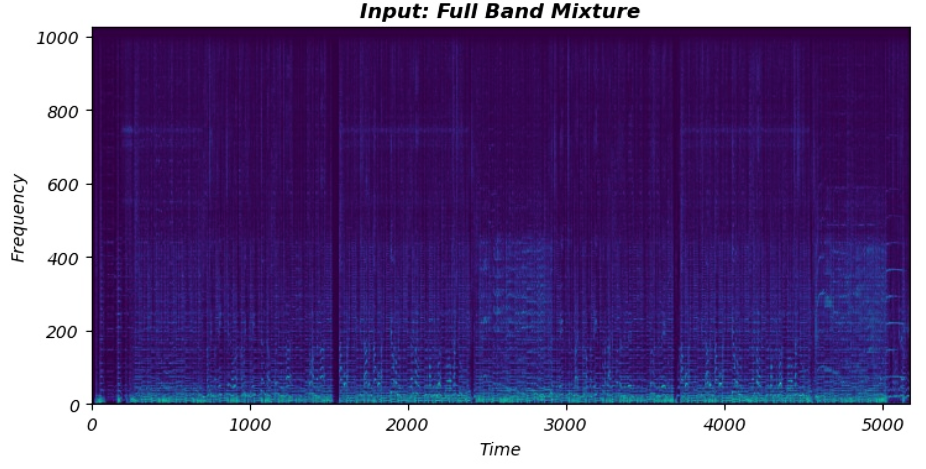
\includegraphics[width=1\linewidth]{Photos/Spectrogram.png}
    \caption{Spectrogram of 'Angels in Amplifiers' from the dataset}
    \label{fig:spectrogram}
\end{figure}



\begin{figure}
    \centering
    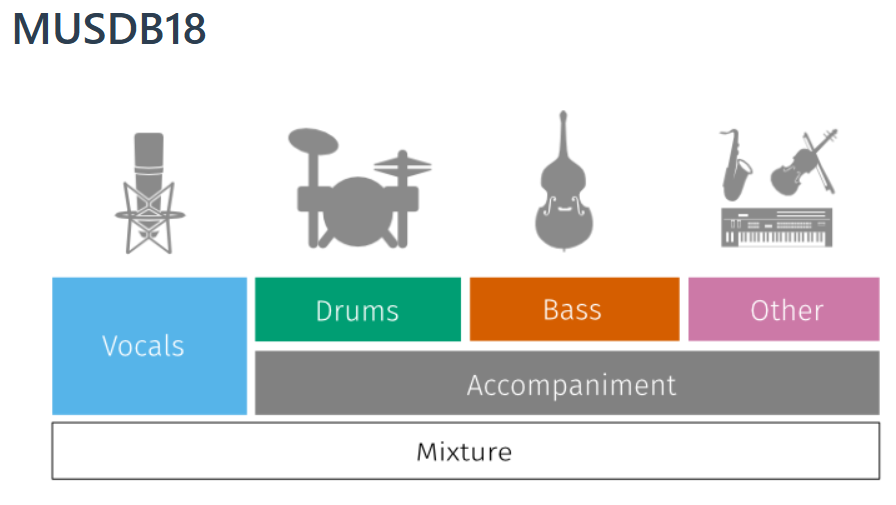
\includegraphics[width=1\linewidth]{Photos/MUSDB.png}
    \caption{MusDB18 tracks}
    \label{fig:musdbtracks}
\end{figure}

\begin{figure}
    \centering
    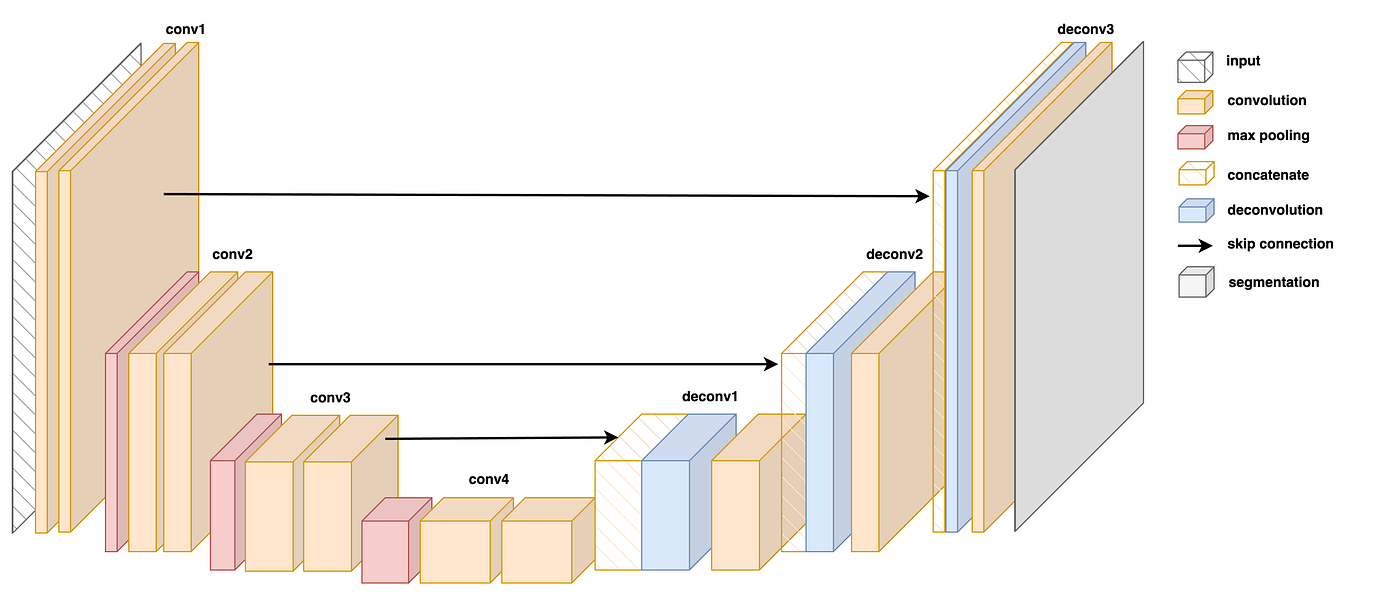
\includegraphics[width=1\linewidth]{Photos/U-Net.png}
    \caption{a U-Net architecture illustration}
    \label{fig:U-Net}
\end{figure}



\end{document}
